\chapter{基于图卷积神经网络的复合物筛选模型}
\label{chapter:NodeConv}

\section{图卷积神经网络介绍}
\label{section:NodeConv:intro}



\section{模型提出}
\label{section:NodeConv:Put}

已有的基于监督学习的复合物预测算法,基本都是基于挖掘复合物子图的拓扑特征,比如图的密度、图的结点个数、平均度数等等,将图的所有拓扑特征置于一个向量中,构成一个$1\times N$的向量,用该向量代替子图,最后将向量用于训练分类模型。具体过程如图\ref{fig:entropy-classification}所示。

\begin{figure}[htbp]
    \centering
    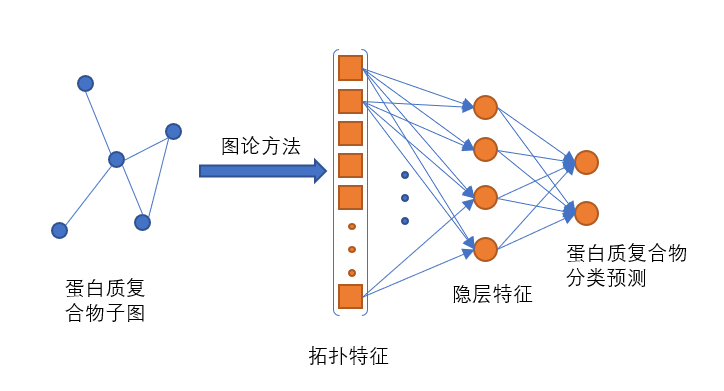
\includegraphics[width=14cm]{entropy-classification}
    \caption{基于图拓扑特征的蛋白质复合物分类模型}
    \label{fig:entropy-classification}
\end{figure}


但是蛋白质复合物中,有大部分复合物是小尺度复合物,其蛋白质个数小于5个。此类复合物的拓扑结构结构简单,提取的拓扑特征具有趋同性。随机的子图在结点数较少的情况下可能形成相同的拓扑特征,此时分类模型无法区分子图是否为真正的复合物。

为了解决该问题,在不引入额外的生物学信息的情况下,本文提出了基于全局特征的复合物分类模型。
蛋白质复合物网络是一个高维结构,可以通过挖掘蛋白质在网络中所处的位置和其周围相互作用关系挖掘蛋白质的潜在特征表示,将网络的高维数据转换为蛋白质的低维嵌入表示,成为每一个蛋白质初始的特征向量。

\section{复合物子图中图卷积神经网络的实现}
\label{section:NodeConv:detail}

本文使用了两种蛋白质特征嵌入模型,分别为Deepwalk和GAE。





\section{算法具体实现与流程}
\label{section:NodeConv:flow}

\begin{figure}[htbp]
    \centering
    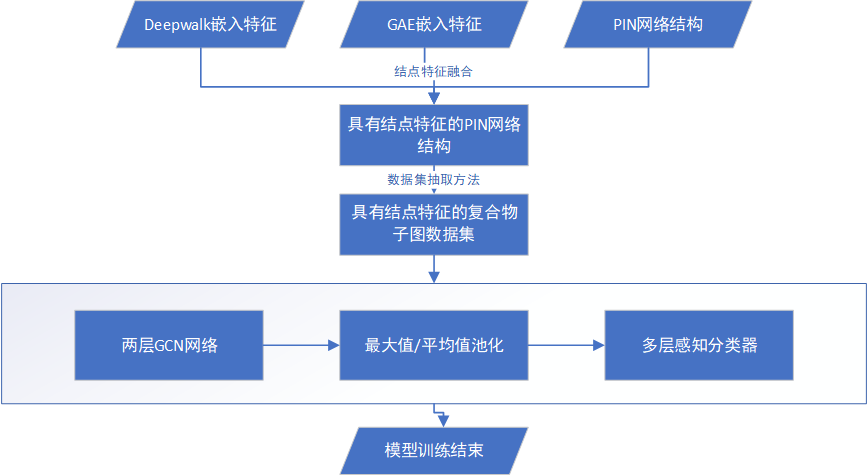
\includegraphics[width=14cm]{node-classification-flow}
    \caption{基于全局特征的分类模型总体流程}
    \label{fig:node-classification-flow}
\end{figure}
基于全局特征的复合物分类模型总体结构如图\ref{fig:node-classification-flow}所示。基于Deepwalk和GAE编码,蛋白质嵌入特征维度总共80维,在$PIN$中加入嵌入特征之后,蛋白质复合物子图具备了初始的结点特征向量。图卷积神经网络\ref{section:NodeConv:intro}具有动态融合结点特征和拓扑结构的能力,已经广泛应用于图任务中。
初始嵌入的80维特征是整个$PIN$网络中结点特征的描述,但是还未结合蛋白质复合物子图的拓扑关系。因此,本文在后续的图分类任务中加上了两层GCN网络对蛋白质结点特征和子图拓扑结构进行融合,增加蛋白质结点特征对复合物内部蛋白质互作关系的描述能力。
最终基于全局特征的复合物分类模型对子图的蛋白质结点特征做平均池化,作为蛋白质复合物特征的输出,以多层感知器预测复合物的分类结果。

\section{实验参数与评估指标}
\label{section:NodeConv:allExperienceDesign}
由于训练数据的不平衡性,训练模型之前,数据进行了重采样处理,保持各分类训练样本相等。按照$8:2$的比率分割各分类样本,形成训练集和测试集。在分类模型的训练过程中,观察训练集和测试集的损失函数,根据早停策略得到未过拟合最佳模型。
本文采用0.001的学习率,batch大小设置为32,隐层维度为128,模型使用了两层的GCN网络以及两层的分类器。
采用LeakyRelu\ref{fig:leakyrelu}作为激活函数和AdamOptimism作为模型优化器。

\begin{figure}[htbp]
    \centering
    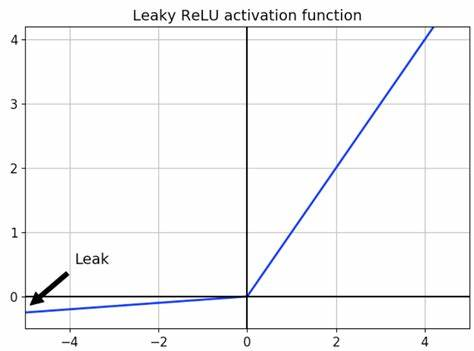
\includegraphics[width=10cm]{leakyrelu}
    \caption{Leaky-Relu 激活函数示意图}
    \label{fig:leakyrelu}
\end{figure}

每一个训练复合物样本都具有复合物类别以及相似性评分两项数据,针对这两项属性,本文实验中分别设置了两项损失函数,使用交叉熵损失(Cross Entropy Loss)计算复合物类别分类损失,使用BCE损失(Binary Cross Entropy Loss)计算复合物得分回归损失。由于两项损失在数值上的差异,设置了相应的损失平衡系数。具体损失计算如下所示。
\begin{equation}
    \label{equ:loss}
    loss=CELoss(PL,TL)+\alpha \cdot BCELoss(PS,TS)
\end{equation}
其中,$PL$为预测类别,$TL$为真实类别,$PS$为预测评分,$TS$为真实评分,$\alpha$为损失平衡系数。

模型测试阶段,本文将复合物生成算法A在$PIN$网络中运行得到算法A预测的复合物$Complexes_A$,用腹黑谁分类模型筛选所有预测结果,其中如果预测样本在筛选模型中被分类为真样本或者评分高于0.25时,预测样本即可通过筛选。最后所有通过筛选的复合物形成复合物集合$Complexes_A'$。最后使用F1值和PPV指标评估$Complexes_A$和$Complexes_A'$的复合物质量。
评价复合物预测结果的常用指标为精准率(precision)、召回率(recall)和F1值(F1-score)。预测复合物和标准复合物计算邻居相似性(NA-similarity)\ref{equ:compComplexSim:NA},计算方式如下所示。
\begin{equation}
    \label{equ:compComplexSim:NA}
    NA_{(\mathcal{P} ,\mathcal{Q} )} = \frac{{\left\lvert V_{\mathcal{P}} \cap V_{\mathcal{Q}}\right\rvert}^2 }{{\left\lvert V_{\mathcal{P}} \right\rvert}\cdot  {\left\lvert V_{\mathcal{Q}} \right\rvert}}
\end{equation}
其中$\mathcal{P}=(V_{\mathcal{P}} ,E_{\mathcal{P}})$是预测复合物,$V_{\mathcal{P}}$为复合物中的蛋白质,$E_{\mathcal{P}}$为复合物中的相互作用,$\mathcal{Q}=(V_{\mathcal{Q}} ,E_{\mathcal{Q}})$是标准复合物。

按照一般性标准,邻居相似性大于0.25时,预测复合物和标准复合物具有匹配性,表示复合物预测成功。
精准率计算如公式\ref{equ:precision}所示。
其中$PC$为预测复合物集合,$M_{PC}$为预测复合物中具有匹配性的所有复合物集合。精准率表示预测复合物中,预测成功的样本所占比重,衡量预测结果的“查准率”。
召回率段计算如公式\ref{equ:recall}所示。
其中$BC$为标准复合物集合,$M_{BC}$为标准复合物中被预测复合物匹配的集合。召回率表示标准复合物中,能被预测复合物匹配的样本所占的比重,衡量预测结果的“查全率”。
F1值综合考虑查准率和查全率,计算如公式\ref{equ:f1}所示。
从定义看出,当查准率和查全率中有一项指标偏小时,F1值就会偏小。
\begin{equation}
    \label{equ:precision}
    precision=\frac{\left\lvert M_{PC}\right\rvert }{\left\lvert PC\right\rvert }
\end{equation}
\begin{equation}
    \label{equ:recall}
    recall=\frac{\left\lvert M_{BC}\right\rvert }{\left\lvert BC\right\rvert }
\end{equation}
\begin{equation}
    \label{equ:f1}
    f-score=\frac{2\times precision\times recall}{precision + recall }
\end{equation}

除此之外,研究者还提出了多种评价复合物预测质量的指标\cite{shi_protein_2011},包括Sn值、PPV值(Cluster-wise Positive Predictive Value)和Acc值等等。

Sn值具体计算方式图式\ref{equ:Sn}所示,
\begin{equation}
    \label{equ:Sn}
    S_n=\frac{\sum_{i = 1}^{n} \max_{j=1}^{m} t_{ij}}{\sum_{i = 1}^{n}n_i}
\end{equation}
其中${j| 1,2,\dots,m }$表示所有的预测复合物,${i| 1,2,\dots,n }$表示所有的标准复合物,$t_{ij}$表示两个复合物$i,j$之间共同蛋白质的数量,$n_i$表示真实复合物中蛋白质的个数。$S_n$值可以反应真实复合物中蛋白质分子被匹配到个数的平均值。

PPV值具体计算方式如式\ref{equ:PPV}所示,
\begin{equation}
    \label{equ:PPV}
    PPV=\frac{\sum_{j = 1}^{m} \max_{i=1}^{n} t_{ij}}{\sum_{i = 1}^{n} \sum_{j = 1}^{m}   t_{ij}}
\end{equation}
可以看出PPV值反应了预测的复合物的匹配程度,PPV值越高,表示预测复合物和标准复合物的平均重合度越高。

Acc值综合考虑了Sn值和PPV值的结果,能更全面的反应预测复合物集合的质量,其具体计算方法如式\ref{equ:Acc}所示。通常情况下,可以将Sn值、PPV值和Acc值的和作为综合的衡量指标\ref{equ:SPA}。
\begin{equation}
    \label{equ:Acc}
    Acc=\sqrt{S_n\times PPV}
\end{equation}

\begin{equation}
    \label{equ:SPA}
    SPA= Sn+PPV+Acc
\end{equation}

\section{实验设计及结果分析}
\label{section:NodeConv:experience}

本章提出了基于全局特征的复合物筛选模型,该模型使用蛋白质网络得到蛋白质编码,在复合物子图中使用GCN网络将蛋白质编码和子图拓扑结构进行融合。
该模型未引入额外的生物学信息,为了验证模型的有效性,本文进行了如下的对比试验。

第一个对比的模型是使用随机特征GCN图分类模型,子图GCN网络输入的结点特征为随机数据,通过该模型的对比验证全局特征的有效性。

第二个对比的模型是采用图论拓扑特征的分类模型\ref{fig:entropy-classification}。计算若干维度的图拓扑特征并进行标准化处理,作为子图特征的代表,用于后续多层感知器分类模型的输入。具体特征提取拓扑特征如表\ref{tab:datasets:statisticgraphfeat}所示。

\begin{table}[h]
    \centering
    \caption{图拓扑特征统计}
    \label{tab:datasets:statisticgraphfeat}
    \begin{tabular}{C{3cm}C{2cm}L{8cm}}
        \toprule
        \textbf{拓扑特征类型} & \textbf{维数} & \textbf{具体描述}                \\
        \midrule
        图总体特征            & 2             & 图结点数,图密度                 \\
        度分布特征            & 4             & 度数平均值、最大值、最小值、方差 \\
        聚类系数特征          & 3             & 聚类系数最大值、平均值、方差     \\
        其他特征              & 1             & 度同配型(degree assortativity) \\
        \bottomrule
    \end{tabular}
\end{table}

图\ref{fig:result/DIP/node}为在DIP网络中,随机结点特征模型、图论拓扑特征模型以及全局特征模型筛选之后结果的对比。
\begin{figure}[htbp]
    \centering
    \subcaptionbox{F1值对比}{\label{fig:result/DIP/F1/node}
        \includegraphics[width=10cm]{result/DIP/F1/node}}
    \vskip0.2cm
    \subcaptionbox{SPA值对比}{\label{fig:result/DIP/SPA/node}
        \includegraphics[width=10cm]{result/DIP/SPA/node}}
    \caption{DIP网络不同模型处理后结果对比}
    \label{fig:result/DIP/node}
\end{figure}

从图中可以看出在DIP网络中随机GCN筛选和基于拓扑GCN筛选可能导致F1值的降低和评价指标的降低,这个原因可能是简单模型在学习的过程中会直接学习直观的拓扑关系,导致分类的错误率较高,在筛选过程中会错误的剔除正样本,导致筛选之后样本质量反而降低。

全局特征的GCN筛选方法,在三个方法中均取得了最佳的F1值和SPA值,证明了全局特征的有效性。

图\ref{fig:result/Biogrid/node}为在Biogrid网络中,随机结点特征模型、图论拓扑特征模型以及全局特征模型筛选之后结果的对比。
\begin{figure}[htbp]
    \centering
    \subcaptionbox{F1值对比}{\label{fig:result/Biogrid/F1/node}
        \includegraphics[width=10cm]{result/Biogrid/F1/node}}
    \vskip0.2cm
    \subcaptionbox{SPA值对比}{\label{fig:result/Biogrid/SPA/node}
        \includegraphics[width=10cm]{result/Biogrid/SPA/node}}
    \caption{Biogrid网络不同模型处理后结果对比}
    \label{fig:result/Biogrid/node}
\end{figure}

从图中可以看出全局特征的GCN筛选对Clique算法的提升十分显著,原因是Clique算法是一种基于3-clique结构挖掘复合物的算法,该算法是一种基于密集连边发现复合物的算法,在Biogrid网络中,网络密度相较于DIP网络高了5.2,因此在Biogrid网络中,Clique算法会相应的产生更多的样本,从而为算法优化提供空间。

从上述结果可以得出。全局特征的GCN筛选方法对原始的样本数据的评价指标都有不同程度的提升。

\section{本章小结}
\label{section:NodeConv:summary}